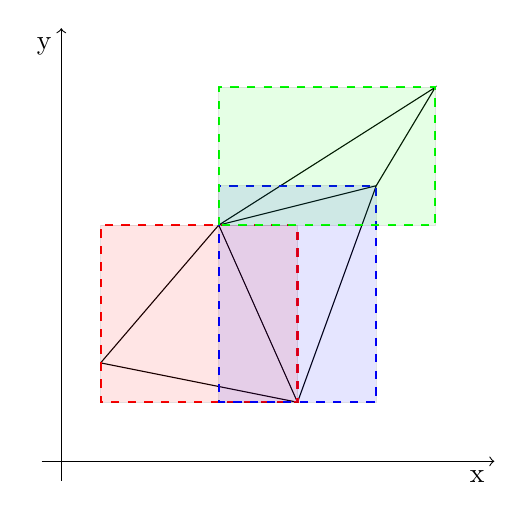
\begin{tikzpicture}[scale=5]
  % axes
	\draw[thin, <->] (1.1,0) node[below left]{x} -| (0, 1.1) node[below left]{y};
  \draw[thin, -] (-0.05,0) -| (0,-0.05);
  
  % mesh
  \coordinate (A) at (0.1, 0.25);
  \coordinate (B) at (0.6, 0.15);
  \coordinate (C) at (0.4, 0.6);
  
  \coordinate (D) at (0.8, 0.7);
  
  \coordinate (E) at (0.95, 0.95);
  
  \draw[thin, -] (A) -- (B) -- (C) -- (A);
  \draw[thin, -] (C) -- (D) -- (B);
  \draw[thin, -] (C) -- (E) -- (D);
  
  %\fill[red] (A) circle(.2pt);
  %\fill[red] (B) circle(.2pt);
  %\fill[red] (C) circle(.2pt);
  %\fill[red] (D) circle(.2pt);
  %\fill[red] (E) circle(.2pt);
  
  % bounding boxes (fill not elegant, but need to get it done)
  \draw[thick, dashed, red]     (A) |- (B) |- (C) -| (A);
  \draw[fill=red, opacity=.1]   (A) |- (B) |- (C) -| (A);
  \draw[thick, dashed, blue]    (C) |- (D) |- (B) -| (C);
  \draw[fill=blue, opacity=.1]  (C) |- (D) |- (B) -| (C);
  \draw[thick, dashed, green]   (C) |- (E) |- (C);
  \draw[fill=green, opacity=.1] (C) |- (E) |- (C);
\end{tikzpicture}